% Created 2016-06-21 Tue 09:34
\documentclass[presentation,smaller]{beamer}
\RequirePackage{etex}
\RequirePackage[l2tabu,orthodox]{nag}            %% Warn about obsolete commands and packages
\RequirePackage{amsmath,amsfonts,amssymb,amsthm} %% Math
\RequirePackage{ifxetex,ifluatex}                %% Detect XeTeX and LuaTeX
\RequirePackage{fixltx2e}                        %% provides \textsubscript
\RequirePackage{xspace}
\RequirePackage{graphicx}
\RequirePackage{comment}
\RequirePackage{url}
\RequirePackage{relsize}
\RequirePackage{booktabs}
\RequirePackage{tabularx}
\RequirePackage[normalem]{ulem}
\RequirePackage[all]{xy}

%%%
%%% Code Listings
%%%

\RequirePackage{listings}
\lstdefinelanguage{Sage}[]{Python}{morekeywords={True,False,sage,cdef,cpdef,ctypedef,self},sensitive=true}

\lstset{frame=none,
  showtabs=False,
  showspaces=False,
  showstringspaces=False,
  commentstyle={\color{gray}},
  keywordstyle={\color{mLightBrown}\textbf},
  stringstyle ={\color{mDarkBrown}},
  frame=single,
  basicstyle=\tt\scriptsize\relax,
  backgroundcolor=\color{gray!190!black},
  inputencoding=utf8,
  literate={…}{{\ldots}}1,
  belowskip=0.0em,
}

%%%
%%% Tikz
%%%

\RequirePackage{tikz,pgfplots}

\usetikzlibrary{calc}
\usetikzlibrary{arrows}
\usetikzlibrary{automata}
\usetikzlibrary{positioning}
\usetikzlibrary{decorations.pathmorphing}
\usetikzlibrary{backgrounds}
\usetikzlibrary{fit,}
\usetikzlibrary{shapes.symbols}
\usetikzlibrary{chains}
\usetikzlibrary{shapes.geometric}
\usetikzlibrary{shapes.arrows}
\usetikzlibrary{graphs}

%% Cache

\ifdefined\tikzcaching  % chktex 1
  \usetikzlibrary{external}
  \tikzexternalize[prefix=build/]
  \tikzset{external/up to date check=diff}  %% MD5 fails from within emacs
\fi

%%%
%%% SVG (Inkscape)
%%%

\ifxetex % chktex 1
\newcommand{\executeiffilenewer}[3]{%
  {\immediate\write18{#3}} % hack
}
\else
\newcommand{\executeiffilenewer}[3]{%
  \ifnum\pdfstrcmp{\pdffilemoddate{#1}}%
    {\pdffilemoddate{#2}}>0%
    {\immediate\write18{#3}}
  \fi%
}
\fi

\newcommand{\includesvg}[2][1.0\textwidth]{%
 \executeiffilenewer{#1.svg}{#1.pdf}%
 {inkscape -z -D --file=#2.svg --export-pdf=#2.pdf --export-latex --export-area-page}%
 \def\svgwidth{#1} 
 \input{#2.pdf_tex}%
} 

%%%
%%% Metropolis Theme
%%%

\usetheme{metropolis}
\metroset{color/block=fill}
\metroset{numbering=none}
\metroset{outer/progressbar=foot}
\metroset{titleformat=smallcaps}

\setbeamercolor{description item}{fg=mLightBrown}
% \setbeamerfont{alerted text}{series=\bfseries}
\setbeamerfont{footnote}{size=\scriptsize}
\setbeamercolor{example text}{fg=mDarkBrown}

\renewcommand*{\UrlFont}{\ttfamily\smaller\relax}

%%%
%%% UTF-8
%%% 

\RequirePackage{unicodesymbols} % after metropolis which loads fontspec

%%%
%%% BibLaTeX
%%%

\RequirePackage[backend=bibtex,
            style=alphabetic,
            maxnames=4,
            citestyle=alphabetic]{biblatex}

\bibliography{local.bib,abbrev3.bib,crypto_crossref.bib}

\DeclareFieldFormat{title}{\alert{#1}}
\DeclareFieldFormat[book]{title}{\alert{#1}}
\DeclareFieldFormat[thesis]{title}{\alert{#1}}
\DeclareFieldFormat[inproceedings]{title}{\alert{#1}}
\DeclareFieldFormat[article]{title}{\alert{#1}}
\DeclareFieldFormat[misc]{title}{\alert{#1}}

%%%
%%% Math Notation
%%% 


\usepackage[landau,probability,logic,complexity,asymptotics]{cryptocode}
\renewcommand{\secpar}{\ensuremath{\lambda}\xspace}

%%% 
%%% Microtype
%%%

\IfFileExists{upquote.sty}{\RequirePackage{upquote}}{}
\IfFileExists{microtype.sty}{\RequirePackage{microtype}}{}

\setlength{\parindent}{0pt}                   %%
\setlength{\parskip}{6pt plus 2pt minus 1pt}  %%
\setlength{\emergencystretch}{3em}            %% prevent overfull lines
\setcounter{secnumdepth}{0}                   %%

%%%
%%% Table of Contents
%%%

\AtBeginSection[] {
  \begin{frame}<beamer>
    \frametitle{Outline}
    \tableofcontents[currentsection]
  \end{frame}
}

%%% Local Variables:
%%% mode: latex
%%% End:
\usepackage{fixltx2e}
\usepackage{graphicx}
\usepackage{grffile}
\usepackage{longtable}
\usepackage{wrapfig}
\usepackage{rotating}
\usepackage[normalem]{ulem}
\usepackage{amsmath}
\usepackage{textcomp}
\usepackage{amssymb}
\usepackage{capt-of}
\usepackage{hyperref}
\usepackage{units}
\usepackage{nicefrac}
\usepackage{gensymb}
\usepackage{amsmath}
\usepackage{amssymb}
\usepackage{xcolor}
\usepackage{listings}
\usetheme{default}
\author{Martin R. Albrecht}
\date{20/06/2016}
\title{fpylll}
\hypersetup{
pdfauthor={Martin R. Albrecht},
pdftitle={fpylll},
pdfkeywords={},
pdfsubject={},
pdfcreator={Emacs 24.5.1 (Org mode 8.3.4)},
pdflang={English},
colorlinks,
citecolor=gray,
filecolor=gray,
linkcolor=gray,
urlcolor=gray
}
\begin{document}

\maketitle

\begin{frame}[label={sec:orgheadline1}]{fpylll}
\begin{itemize}
\item \href{https://github.com/malb/fpylll}{fpylll} is a Python library for performing lattice reduction on lattices over the Integers.
\item It is based on the \href{https://github.com/dstehle/fplll}{fplll}
\item fpylll also implements a few algorithms beyond fplll and provides some interface niceties
\end{itemize}

\begin{block}{Mission}
Make implementing lattice-reduction strategies so easy, we can demand people to publish their code.
\end{block}
\end{frame}

\begin{frame}[label={sec:orgheadline2}]{fpylll}
\begin{itemize}
\item \href{https://github.com/malb/fpylll}{fpylll} is a Python library for performing lattice reduction on lattices over the Integers.
\item It is based on the \href{https://github.com/dstehle/fplll}{fplll}
\item fpylll also implements a few algorithms beyond fplll and provides some interface niceties
\end{itemize}

\begin{block}{Mission}
Make implementing lattice-reduction strategies so easy, even I can do it.
\end{block}
\end{frame}

\begin{frame}[fragile,label={sec:orgheadline3}]{Highlevel Interface}
 First of all, \alert{fpylll} is a thin wrapper around \alert{fplll}. In the example below, we first generate an NTRU-like matrix and consider the norm of the first row:

\lstset{language=Python,label= ,caption= ,captionpos=b,numbers=none}
\begin{lstlisting}
from fpylll import IntegerMatrix, LLL
q = 1073741789
A = IntegerMatrix.random(30, "ntrulike", bits=30, q=q)
A[0].norm()
\end{lstlisting}

3294809651.09
\end{frame}

\begin{frame}[fragile,label={sec:orgheadline4}]{Highlevel Interface}
 We then call \href{https://en.wikipedia.org/wiki/Lenstra–Lenstra–Lovász_lattice_basis_reduction_algorithm}{LLL reduction} and observe the output:

\lstset{language=Python,label= ,caption= ,captionpos=b,numbers=none}
\begin{lstlisting}
LLL.reduction(A)
A[0].norm()
\end{lstlisting}

82117.5815888
\end{frame}

\begin{frame}[fragile,label={sec:orgheadline5}]{Highlevel Interface}
 If LLL reduction isn’t strong enough, we can call the BKZ algorithm for some block size \(k\).

\lstset{language=Python,label= ,caption= ,captionpos=b,numbers=none}
\begin{lstlisting}
from fpylll import BKZ
BKZ.reduction(A, o=BKZ.Param(block_size=10))
A[0].norm()
\end{lstlisting}

71600.8858744
\end{frame}

\begin{frame}[fragile,label={sec:orgheadline6}]{Highlevel Interface}
 Or SVP directly.

\lstset{language=Python,label= ,caption= ,captionpos=b,numbers=none}
\begin{lstlisting}
from fpylll import SVP
q = 1073741789
B = IntegerMatrix.random(10, "ntrulike", bits=7, q=127)
SVP.shortest_vector(B)
\end{lstlisting}

(0, 2, -6, -6, 0, 0, 3, 2, -5, 1, 0, 5, -5, -3, 0, -1, -3, 3, -5, -7)
\end{frame}

\begin{frame}[fragile,label={sec:orgheadline7}]{Lowlevel Interface}
 \lstset{language=Python,label= ,caption= ,captionpos=b,numbers=none}
\begin{lstlisting}
from fpylll import IntegerMatrix, GSO
q = 1073741789
A = IntegerMatrix.random(30, "ntrulike", bits=30, q=q)
M = GSO.Mat(A)
M.update_gso()
\end{lstlisting}

True


\lstset{language=Python,label= ,caption= ,captionpos=b,numbers=none}
\begin{lstlisting}
M.get_r(0,0)
\end{lstlisting}

1.26228336805e+19
\end{frame}

\begin{frame}[fragile,label={sec:orgheadline8}]{Lowlevel Interface}
 \lstset{language=Python,label= ,caption= ,captionpos=b,numbers=none}
\begin{lstlisting}
A[2][3] + 2*A[3][3]
\end{lstlisting}

2

\lstset{language=Python,label= ,caption= ,captionpos=b,numbers=none}
\begin{lstlisting}
with M.row_ops(2,4):
    M.row_addmul(2,3,2)
\end{lstlisting}

\lstset{language=Python,label= ,caption= ,captionpos=b,numbers=none}
\begin{lstlisting}
A[2][3]
\end{lstlisting}

2
\end{frame}

\begin{frame}[fragile,label={sec:orgheadline9}]{Coverage}
 \begin{verbatim}
bkz.pyx
enumeration.pyx
gso.pyx
integer_matrix.pyx
lll.pyx
svpcvp.pyx
wrapper.pyx
\end{verbatim}
\end{frame}

\begin{frame}[label={sec:orgheadline10}]{Multicore}
Of course, \alert{fpylll} being a Python library means you can use your favourite Python libraries with it. 

For example, say, we want to LLL reduce many matrices in parallel, using all our cores, and to compute the norm of the shortest vector across all matrices after LLL reduction. 
\end{frame}

\begin{frame}[fragile,label={sec:orgheadline11}]{Multicore}
 We’ll make use of Python’s \href{https://docs.python.org/2/library/multiprocessing.html}{multiprocessing}:

\lstset{language=Python,label= ,caption= ,captionpos=b,numbers=none}
\begin{lstlisting}
from multiprocessing import Pool
\end{lstlisting}

For this example, we want dimension 40, four worker processes and 32 matrices:

\lstset{language=Python,label= ,caption= ,captionpos=b,numbers=none}
\begin{lstlisting}
from fpylll import *
q = 1073741789
workers = 4
tasks = 32
A  = []

for i in range(tasks):
    A.append(IntegerMatrix.random(20, "ntrulike", bits=30, q=q))
\end{lstlisting}

32
\end{frame}

\begin{frame}[fragile,label={sec:orgheadline12}]{Multicore}
 Let’s get to work: we create a pool of workers and kick off the computation:

\lstset{language=Python,label= ,caption= ,captionpos=b,numbers=none}
\begin{lstlisting}
pool = Pool(workers)
A = pool.map(LLL.reduction, A)
\end{lstlisting}

Finally, we output the minimal norm found:

\lstset{language=Python,label= ,caption= ,captionpos=b,numbers=none}
\begin{lstlisting}
min([A_[0].norm() for A_ in A])
\end{lstlisting}

7194.54515588
\end{frame}

\begin{frame}[fragile,label={sec:orgheadline13}]{Plotting}
 \lstset{language=Python,label= ,caption= ,captionpos=b,numbers=none}
\begin{lstlisting}
from fpylll import IntegerMatrix, GSO
from math import log
q = 1073741789
A = IntegerMatrix.random(40, "ntrulike", bits=30, q=q)
M = GSO.Mat(A)
M.update_gso()
gso = [log(M.get_r(i,i)) for i in range(40)]
\end{lstlisting}

True
\end{frame}

\begin{frame}[fragile,label={sec:orgheadline14}]{Plotting}
 \lstset{language=Python,label= ,caption= ,captionpos=b,numbers=none}
\begin{lstlisting}
import matplotlib
import matplotlib.pyplot as plt
plt.plot(gso)
plt.savefig('gso.png')
'gso.png' # return this to org-mode
\end{lstlisting}

\begin{center}
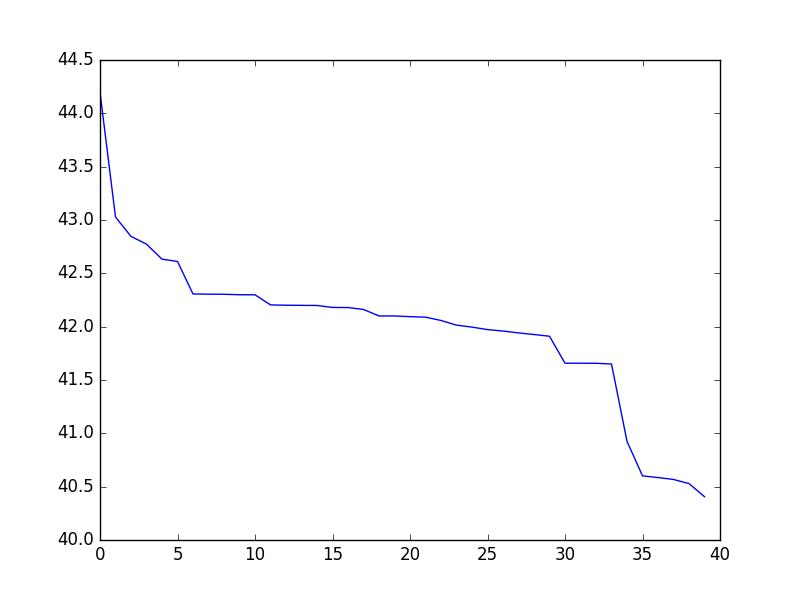
\includegraphics[width=0.5\textwidth]{gso.png}
\end{center}
\end{frame}

\begin{frame}[label={sec:orgheadline15}]{Developing Lattice-Reduction Algorithms}
\begin{itemize}
\item The main objective of \alert{fpylll} is to make developing and experimenting with the kind of algorithms implemented in \alert{fplll} easier.
\item For example, there are a few variants of the BKZ algorithm in the literature which essentially re-combine the same building blocks — LLL and an SVP oracle — in some way.
\item These kind of algorithms should be easy to implement.
\end{itemize}

The code below is an implementation of the \href{https://github.com/malb/fpylll/blob/master/src/fpylll/contrib/simple_bkz.py}{plain BKZ algorithm} in 70 lines of Python.
\end{frame}

\begin{frame}[fragile,label={sec:orgheadline16}]{BKZ}
 \lstset{language=Python,label= ,caption= ,captionpos=b,numbers=none}
\begin{lstlisting}
from fpylll import IntegerMatrix, GSO, LLL, BKZ
from fpylll import Enumeration as Enum
from fpylll import gso
\end{lstlisting}
\end{frame}

\begin{frame}[fragile,label={sec:orgheadline17}]{BKZ}
 \lstset{language=Python,label= ,caption= ,captionpos=b,numbers=none}
\begin{lstlisting}
class BKZReduction:
    def __init__(self, A):
        wrapper = LLL.Wrapper(A)
        wrapper()

        self.A = A
        self.M = GSO.Mat(A, flags=gso.GSO.ROW_EXPO)
        self.lll_obj = LLL.Reduction(self.M)
\end{lstlisting}
\end{frame}

\begin{frame}[fragile,label={sec:orgheadline18}]{BKZ}
 \lstset{language=Python,label= ,caption= ,captionpos=b,numbers=none}
\begin{lstlisting}
    def __call__(self, block_size):
        self.M.discover_all_rows()

        while True:
            clean = self.tour(block_size, 0, self.A.nrows)
            if clean:
                break
\end{lstlisting}
\end{frame}

\begin{frame}[fragile,label={sec:orgheadline19}]{BKZ}
 \lstset{language=Python,label= ,caption= ,captionpos=b,numbers=none}
\begin{lstlisting}
    def tour(self, block_size, min_row, max_row):
        clean = True
        for kappa in range(min_row, max_row-1):
            bs = min(block_size, max_row - kappa)
            clean &= self.svp_reduction(kappa, bs)
        return clean
\end{lstlisting}
\end{frame}

\begin{frame}[fragile,label={sec:orgheadline20}]{BKZ}
 \lstset{language=Python,label= ,caption= ,captionpos=b,numbers=none}
\begin{lstlisting}
    def svp_reduction(self, kappa, block_size):
        clean = True

        self.lll_obj(0, kappa, kappa + block_size)
        if self.lll_obj.nswaps > 0:
            clean = False

        max_dist, expo = self.M.get_r_exp(kappa, kappa)
        delta_max_dist = self.lll_obj.delta * max_dist

        solution, max_dist = Enum.enumerate(self.M, max_dist, expo, \
                                   kappa, kappa + block_size, None)

        if max_dist >= delta_max_dist:
            return clean
\end{lstlisting}
\end{frame}

\begin{frame}[fragile,label={sec:orgheadline21}]{BKZ}
 \lstset{language=Python,label= ,caption= ,captionpos=b,numbers=none}
\begin{lstlisting}
        nonzero_vectors = len([x for x in solution if x])

        if nonzero_vectors == 1:
            first_nonzero_vector = None
            for i in range(block_size):
                if abs(solution[i]) == 1:
                    first_nonzero_vector = i
                    break

            self.M.move_row(kappa + first_nonzero_vector, kappa)
            self.lll_obj.size_reduction(kappa, kappa + 1)
\end{lstlisting}
\end{frame}

\begin{frame}[fragile,label={sec:orgheadline22}]{BKZ}
 \lstset{language=Python,label= ,caption= ,captionpos=b,numbers=none}
\begin{lstlisting}
        else:
            d = self.M.d
            self.M.create_row()

            with self.M.row_ops(d, d+1):
                for i in range(block_size):
                    self.M.row_addmul(d, kappa + i, solution[i])

            self.M.move_row(d, kappa)
            self.lll_obj(kappa, kappa, kappa + block_size + 1)
            self.M.move_row(kappa + block_size, d)

            self.M.remove_last_row()

        return False
\end{lstlisting}
\end{frame}

\begin{frame}[fragile,label={sec:orgheadline23}]{Beyond fplll}
 \begin{itemize}
\item In the meantime \alert{fpylll} has gained a \texttt{contrib} module which implements additional algorithms.
\item As of writing, it contains
\begin{itemize}
\item a simple demo implementation of BKZ (see above),
\item a simple implementation of \href{http://ia.cr/2015/1123}{Dual BKZ} and a slightly feature enhanced re-implementation of fplll’s BKZ which collects additional statistics compared to fplll’s implementation of the same algorithm.
\end{itemize}
\end{itemize}
\end{frame}

\begin{frame}[fragile,label={sec:orgheadline24}]{Beyond fplll}
 \lstset{language=Python,label= ,caption= ,captionpos=b,numbers=none}
\begin{lstlisting}
from copy import copy
from fpylll import BKZ
from fpylll.contrib.bkz import BKZReduction

C = copy(A)
b = BKZReduction(C)
b(BKZ.Param(block_size=30, flags=BKZ.AUTO_ABORT|BKZ.VERBOSE))
stats = b.stats; stats
\end{lstlisting}

\{"i":  25,  "total":     12.01,  "time":     0.40,  "preproc":     0.10,  "svp":     0.10,  "r\(_{\text{0}}\)": 7.3483e+09,  "slope": -0.0538,  "enum nodes": 20.31,  "max(kappa)":   6\}
\end{frame}

\begin{frame}[fragile,label={sec:orgheadline25}]{Beyond fplll}
 That output isn’t that different from \alert{fplll} outputs. However, in contrast to \alert{fplll} (because I didn’t bother to implement it over there, yet) we also get access to a \texttt{stats} object after the computation finished. Let’s use it to inquire how many nodes where visited during enumeration

\lstset{language=Python,label= ,caption= ,captionpos=b,numbers=none}
\begin{lstlisting}
stats.enum_nodes
\end{lstlisting}

39977944

and how much time we spent in enumeration:

\lstset{language=Python,label= ,caption= ,captionpos=b,numbers=none}
\begin{lstlisting}
stats.svp_time
\end{lstlisting}

3.119223
\end{frame}

\begin{frame}[fragile,label={sec:orgheadline26}]{Integration with other Projects}
 \alert{fpylll} integrates reasonably nicely with \href{http://sagemath.org}{Sage}: converting back and forth between data types is seamless. For example:

\lstset{language=sage,label= ,caption= ,captionpos=b,numbers=none}
\begin{lstlisting}
sage: A = random_matrix(ZZ, 10, 10)
sage: from fpylll import IntegerMatrix, LLL
sage: B = IntegerMatrix.from_matrix(A)
sage: LLL.reduction(B)
sage: B.to_matrix(A)[0]
\end{lstlisting}
(-2, 1, 0, -1, 0, 0, 1, -2, 0, 0)
\end{frame}

\begin{frame}[fragile,label={sec:orgheadline27}]{Integration with other Projects}
 In fact, when installed inside Sage, element access for \texttt{IntegerMatrix} accepts and returns \texttt{sage.rings.integer.Integer} directly, instead of Python integers.

\lstset{language=sage,label= ,caption= ,captionpos=b,numbers=none}
\begin{lstlisting}
sage: type(B[0,0])
<type 'sage.rings.integer.Integer'>
\end{lstlisting}
\end{frame}

\begin{frame}[fragile,label={sec:orgheadline28}]{Integration with other Projects}
 \alert{fpylll} also integrates somewhat with \href{http://www.numpy.org}{NumPy}.

\lstset{language=Python,label= ,caption= ,captionpos=b,numbers=none}
\begin{lstlisting}
from fpylll import *
A = IntegerMatrix.random(4, "ntrulike", bits=7, q=127)
\end{lstlisting}

We’d like to do some analysis on its Gram-Schmidt matrix, so let’s compute it:

\lstset{language=Python,label= ,caption= ,captionpos=b,numbers=none}
\begin{lstlisting}
sage: M = GSO.Mat(A)
sage: M.update_gso()
\end{lstlisting}
\end{frame}

\begin{frame}[fragile,label={sec:orgheadline29}]{Integration with other Projects}
 Let’s dump it into a NumPy array and spot check that the result is reasonably close:

\lstset{language=Python,label= ,caption= ,captionpos=b,numbers=none}
\begin{lstlisting}
import numpy
from fpylll.numpy import dump_mu
N = numpy.ndarray(dtype="double", shape=(8,8))
dump_mu(N, M, 0, 8)
N[1,0] - M.get_mu(1,0)
\end{lstlisting}

0.0

Let’s do something more or less useful with our output:

\lstset{language=Python,label= ,caption= ,captionpos=b,numbers=none}
\begin{lstlisting}
numpy.linalg.eigvals(N)
\end{lstlisting}

[ -7.99122854e-40 +0.00000000e+00j  -5.65065189e-40 +5.65065189e-40j
  -5.65065189e-40 -5.65065189e-40j  -8.15663058e-56 +7.99122854e-40j
  -8.15663058e-56 -7.99122854e-40j   7.99122854e-40 +0.00000000e+00j
   5.65065189e-40 +5.65065189e-40j   5.65065189e-40 -5.65065189e-40j]
\end{frame}

\begin{frame}[fragile,label={sec:orgheadline30}]{Tests}
 \alert{fpylll} runs tests on every check-in for Python 2 and 3. As an added benefit, this extends test coverage for \alert{fplll} as well, which only has a few highlevel tests.

\lstset{language=Python,label= ,caption= ,captionpos=b,numbers=none}
\begin{lstlisting}
def test_lll_lll():
    for m, n in dimensions:
        A = make_integer_matrix(m, n)
        b00 = []
        for float_type in float_types:
            B = copy(A)
            M = GSO.Mat(B, float_type=float_type)
            lll = LLL.Reduction(M)
            lll()
            if (m, n) == (0, 0):
                continue
            b00.append(B[0, 0])
        for i in range(1, len(b00)):
            assert b00[0] == b00[i]
\end{lstlisting}
\end{frame}

\begin{frame}[fragile,label={sec:orgheadline31}]{Lisp}
 “This is all nice and well”, I hear you say, “but I prefer to do my computations in Lisp, so thanks, but not thanks”. 

\url{https://imgs.xkcd.com/comics/lisp_cycles.png}

No worries, \href{http://docs.hylang.org/en/latest/}{Hy} has you covered:

\lstset{language=Lisp,label= ,caption= ,captionpos=b,numbers=none}
\begin{lstlisting}
=> (import [fpylll [*]])
=> (setv q 1073741789)
=> (setv A (.random IntegerMatrix 30 "ntrulike" :bits 30 :q q))   
=> (car A)
row 0 of <IntegerMatrix(60, 60) at 0x7f1cbbfbf888>
=> (get A 1)
row 1 of <IntegerMatrix(60, 60) at 0x7f1cbbfbf888>
=> (-> (car A) (.norm))
4019682565.5285482

=> (.reduction LLL A)
=> (.norm (car A))
6937.9845776709535
\end{lstlisting}
\end{frame}

\begin{frame}[label={sec:orgheadline32}]{Help Wanted}
\begin{itemize}
\item \alert{fpylll} isn’t \href{https://github.com/malb/fpylll/issues}{quite done yet}.
\item Besides testing and documentation, it would be nice if someone would attempt to re-implement fplll’s \href{https://github.com/dstehle/fplll/blob/master/src/wrapper.h}{LLL wrapper} in pure Python.
\item This would serve as a test case to see if everything that’s needed really is exposed and as a starting point for others who like to tweak the strategy.
\item Speaking of LLL, \alert{fpylll} is currently somewhat biased towards playing with BKZ, i.e. it would be nice to see how useful it is for trying out tweaks to the LLL algorithm.
\end{itemize}
\end{frame}

\begin{frame}[label={sec:orgheadline33}]{Fin}
\begin{center}
\begin{Huge}
\alert{Thank You}
\end{Huge}
\end{center}
\end{frame}
\end{document}